% Chapter 5

\chapter{Results} % Main chapter title

\label{Chapter5} % For referencing the chapter elsewhere, use~\ref{Chapter5} 

In this research, we use the offline measurement generator in getting the
measurement across different real-world programs. We calculate the ScaRR control
flow information for each of the programs. We analyze and present the result in
this chapter. The analysis and source code of the program is available
online.\footnote{Our offline measurement generator is available here
\url{https://github.com/lamida/scarr-sample-program/}.}

We choose four large open-source software projects for analysis. The first
software is Redis $6.2.4$ ~\cite{RedisRedis2021}, a so-called data structure
server. The Redis source build consists of the server binary and the client
command-line interface (CLI). We analyze both of the programs. The second
program we analyze is bzip2 $1.0.8$~\cite{Bzip2Bzip2}. Bzip2 is a free and
open-source file compression program. The third program is OpenSSL
$1.1.1j$~\cite{OpensslOpenssl2021}. OpenSSL is a full-featured toolkit for TLS
protocol. The last program we analyze is Coreutils
$8.32$~\cite{CoreutilsCoreutils2021}. Coreutils is a suite of Unix utilities for
file, shell, and text manipulation.

\section{Running LLVM Pass}
\label{sec:running-llvm-pass}

We write the tool to extract the ScaRR offline measurement using LLVM.
Specifically, we implement the tool as LLVM pass. We discuss some background on
LLVM pass in Subsection \ref{subsec:llvm-pass} in Chapter~\ref{Chapter3}. In
this section, we show how to use the pass.

\begin{listing}[h]
    \begin{minted}[
        frame=lines,
        framesep=2mm,
        baselinestretch=1.2,
        fontsize=\footnotesize,
    ]{console}
        opt -passes=scarr-cp-marker <file>.ll
    \end{minted}
    \caption{Mark Checkpoint in BasicBlock.}    
    \label{listing:mark-cp-in-cfg}
\end{listing}

\begin{listing}[h]
    \begin{minted}[
        frame=lines,
        framesep=2mm,
        baselinestretch=1.2,
        fontsize=\footnotesize,
    ]{console}
        opt -passes=scarr-cp-marker,dot-cfg <file>.ll
    \end{minted}
    \caption{Print Checkpoints in CFG dot file.}    
    \label{listing:cp-to-cfg}
\end{listing}

\begin{listing}[h]
    \begin{minted}[
        frame=lines,
        framesep=2mm,
        baselinestretch=1.2,
        fontsize=\footnotesize,
    ]{console}
        opt -passes=scarr-cp-marker,scarr-loa-collector <file>.ll
    \end{minted}
    \caption{Get List of Actions.}    
    \label{listing:get-loa}
\end{listing}

\begin{listing}[h]
    \begin{minted}[
        frame=lines,
        framesep=2mm,
        baselinestretch=1.2,
        fontsize=\footnotesize,
    ]{text}
    =============================================================
    ScaRR Offline Measurement Statistics
    =============================================================
    Offline Measurement Size: 151
    Number of Checkpoints: 94
    Number of List of Actions: 216
    csv,../cat.ll,119,151,94,216
    =============================================================
    Checkpoints and LoA Details: 
    ============================================================
    ... the detail output ...
    \end{minted}
    \caption{Output of ScaRR Offline Measurement.}    
    \label{listing:scarr-output}
\end{listing}

We can invoke LLVM \texttt{opt} to mark the list of Checkpoints as shown in
Listing~\ref{listing:mark-cp-in-cfg}. We can see the output of the marked basic
block using LLVM \texttt{dot-cfg} pass. The commands in
Listing~\ref{listing:cp-to-cfg} generates different dot files per function. We
can use \texttt{xdot} command line from Graphiz to see the graph. To mark the
list of actions between checkpoints, we can invoke LLVM \texttt{opt} as shown in
Listing~\ref{listing:get-loa}. Note that we have to run \texttt{scarr-cp-marker}
before \texttt{scarr-loa-collector}. Listing~\ref{listing:scarr-output} shows
output of the offline measurement extractor.

\section{ScaRR Control-Flow Result}

For each program, we collect the following measurements. The text in parenthesis
are the abbreviations that we use for the column headers in
Table~\ref{table:scarr-result}.
In particular, we measured:
\begin{itemize}
    \item Source code lines (CL)
    \item IR lines (IRL)
    \item Number of basic blocks (BB)
    \item Number of ScaRR measurements (M)
    \item Number of checkpoints (CP)
    \item Number of LoA (LoA)
\end{itemize}



\afterpage{
\rowcolors{2}{}{lightgray!20}
\begin{longtable}{lrrrrrr}
    \toprule 
    Program         & CL         & IRL & BB & M & CP & LoA  \\
    \midrule 
    \multicolumn{7}{l}{Coreutils} \\
    \midrule 
    basename        & 190        & 827      & 19              & 17              & 13             & 26       \\
    cat             & 767        & 2215     & 119             & 151             & 94             & 216      \\
    chgrp           & 319        & 1158     & 43              & 44              & 32             & 60       \\
    cksum           & 310        & 1012     & 9               & 11              & 8              & 20       \\
    cp              & 1226       & 3619     & 79              & 37              & 27             & 56       \\
    cut             & 609        & 2196     & 40              & 36              & 25             & 56       \\
    date            & 604        & 2223     & 69              & 80              & 57             & 110      \\
    dd              & 2581       & 9420     & 366             & 451             & 235            & 748      \\
    df              & 1847       & 8146     & 377             & 410             & 278            & 698      \\
    dirname         & 136        & 635      & 13              & 13              & 10             & 20       \\
    du              & 1140       & 3973     & 206             & 273             & 138            & 424      \\
    env             & 952        & 3875     & 197             & 241             & 141            & 374      \\
    expand          & 238        & 1057     & 46              & 55              & 37             & 78       \\
    false           & 2          & 442      & 6               & 7               & 6              & 12       \\
    fmt             & 1029       & 4083     & 44              & 45              & 26             & 64       \\
    getlimits       & 172        & 2681     & 109             & 189             & 109            & 324      \\
    head            & 1095       & 3596     & 196             & 253             & 149            & 386      \\
    id              & 464        & 1922     & 67              & 47              & 31             & 84       \\
    install         & 1059       & 3545     & 120             & 129             & 72             & 162      \\
    kill            & 314        & 1376     & 64              & 90              & 49             & 142      \\
    link            & 93         & 581      & 10              & 8               & 8              & 12       \\
    ln              & 681        & 2350     & 64              & 60              & 37             & 100      \\
    ls              & 5520       & 24925    & 394             & 450             & 249            & 654      \\
    make-prime-list & 230        & 813      & 32              & 43              & 27             & 78       \\
    mkdir           & 296        & 1230     & 28              & 30              & 21             & 42       \\
    mktemp          & 350        & 1347     & 65              & 80              & 53             & 120      \\
    mv              & 512        & 1903     & 66              & 61              & 40             & 92       \\
    nice            & 221        & 905      & 27              & 31              & 24             & 54       \\
    nl              & 596        & 1994     & 35              & 39              & 24             & 58       \\
    numfmt          & 1651       & 6036     & 113             & 118             & 69             & 154      \\
    od              & 1987       & 7876     & 230             & 291             & 173            & 454      \\
    paste           & 530        & 2234     & 31              & 41              & 27             & 54       \\
    pathchk         & 422        & 1306     & 56              & 77              & 44             & 120      \\
    pinky           & 602        & 3161     & 72              & 84              & 48             & 128      \\
    pr              & 2848       & 10596    & 105             & 89              & 50             & 142      \\
    printenv        & 154        & 742      & 25              & 34              & 20             & 60       \\
    printf          & 715        & 2811     & 118             & 147             & 92             & 200      \\
    ptx             & 2153       & 7888     & 487             & 651             & 294            & 1060     \\
    pwd             & 394        & 1777     & 65              & 74              & 50             & 116      \\
    readlink        & 178        & 813      & 34              & 36              & 24             & 50       \\
    realpath        & 278        & 1382     & 74              & 86              & 49             & 134      \\
    rm              & 373        & 1213     & 40              & 41              & 26             & 64       \\
    rmdir           & 253        & 1048     & 31              & 38              & 23             & 62       \\
    seq             & 736        & 3057     & 105             & 132             & 84             & 226      \\
    shred           & 1279       & 3789     & 67              & 83              & 52             & 130      \\
    shuf            & 615        & 2524     & 128             & 177             & 106            & 310      \\
    sleep           & 146        & 688      & 21              & 28              & 18             & 46       \\
    split           & 1668       & 6262     & 248             & 302             & 189            & 510      \\
    stat            & 1907       & 18653    & 55              & 65              & 44             & 86       \\
    stdbuf          & 394        & 1644     & 87              & 109             & 76             & 154      \\
    stty            & 2322       & 5885     & 163             & 167             & 110            & 250      \\
    sum             & 273        & 1312     & 15              & 19              & 14             & 32       \\
    sync            & 239        & 838      & 29              & 39              & 27             & 58       \\
    tac             & 713        & 2324     & 64              & 75              & 48             & 116      \\
    tail            & 2537       & 8657     & 458             & 575             & 329            & 894      \\
    tee             & 278        & 1193     & 48              & 61              & 37             & 96       \\
    tr              & 1914       & 6139     & 152             & 167             & 97             & 282      \\
    true            & 80         & 441      & 6               & 7               & 6              & 12       \\
    truncate        & 388        & 1564     & 78              & 94              & 58             & 150      \\
    tty             & 133        & 624      & 13              & 14              & 12             & 20       \\
    uname           & 376        & 1236     & 76              & 101             & 61             & 140      \\
    unexpand        & 326        & 1255     & 60              & 67              & 46             & 98       \\
    uniq            & 662        & 2379     & 110             & 125             & 77             & 192      \\
    unlink          & 88         & 543      & 7               & 5               & 6              & 10       \\
    uptime          & 257        & 1249     & 5               & 2               & 3              & 4        \\
    users           & 150        & 899      & 5               & 2               & 3              & 4        \\
    wc              & 895        & 3689     & 89              & 100             & 68             & 158      \\
    yes             & 130        & 765      & 19              & 26              & 15             & 44       \\
    \midrule 
    \multicolumn{7}{l}{Redis} \\
    \midrule 
    redis-benchmark & 1982       & 29367    & 254             & 407             & 211            & 564       \\
    redis-cli       & 8400       & 45836    & 513             & 630             & 388            & 1002       \\
    server          & 6397       & 25790    & 88              & 91              & 52             & 138       \\
    \midrule 
    \multicolumn{7}{l}{Bzip2} \\
    \midrule 
    bzip2           & 2036       & 8542    & 143             & 132             & 76            & 244       \\
    \midrule 
    \multicolumn{7}{l}{OpenSSL} \\
    \midrule 
    openssl         & 832        & 1793    & 28              & 30              & 19            & 42       \\
    \bottomrule
    \caption{ScaRR Offline Measurement Result.}
    \label{table:scarr-result}
    \end{longtable}
\rowcolors{2}{}{}
}

We can see the trend from the measurement in the table by sorting the data
first. Figure~\ref{fig:measurement-result} presents the measurements result by
comparing the number of basic blocks against three different measurement
metrics: number of checkpoints, number of LoAs and number of measurements. We
can see there is a linear relationship among the metrics, which verifies
our assumption.


\begin{figure}[t]
    \centerline{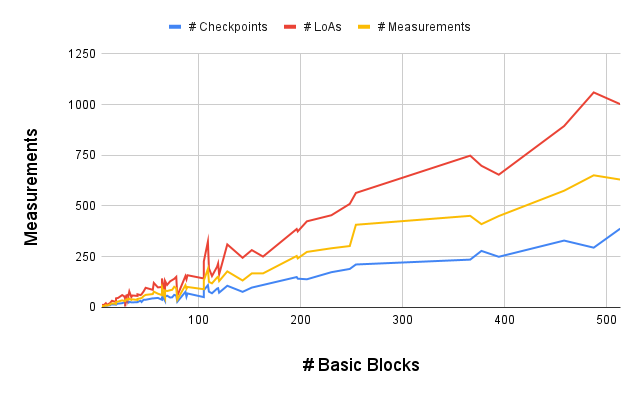
\includegraphics[scale=.65]{Figures/05/scarr-result-v2.png}}
    \caption{Measurement Results.} 
    \label{fig:measurement-result}
\end{figure}


\section{Complexity Analysis}

We split the complexity analysis of the program into time complexity and space
complexity. The time complexity of Checkpoint Marker is $O(n)$. We only need to
traverse the basic block once to identify whether a basic block is a checkpoint.
The time complexity of LoA collector is also $O(n)$. We traverse the basic block
one time either by breadth-first or depth-first list of the basic block. First,
we mark the first checkpoint as the first basic block as we move in traversing.
We stop as soon as we find the next checkpoint or a first basic block after
branch. We can see the time complexity of LoA collector is $O(n)$.

The space complexity for both algorithms is also $O(n)$. The only additional
storage that we require is to store N number basic block during marking the
checkpoint and then collecting the LoA.

\section{Case Study}

We present a simple case study on how we process a program and
get the offline measurement. We consider a program in
Listing~\ref{listing:simple-loop}. The IR is in the
Listing~\ref{listing:simple-loop-ir}. We can see the basic block of the program
in Figure~\ref{fig:simple-loop-bb}. 


\begin{listing}[h]
    \begin{minted}[
        frame=lines,
        framesep=2mm,
        baselinestretch=1.2,
        fontsize=\footnotesize,
        ]{c}
        int main() {
            for (int i = 0; i < 10; i++) {
                // do nothing
            }
        }
    \end{minted}
    \caption{Case Study Program.}    
    \label{listing:simple-loop}
\end{listing}

\begin{listing}[h]
    \inputminted[
    frame=lines,
    framesep=2mm,
    baselinestretch=1.2,
    fontsize=\footnotesize,
    linenos
    ]{c}{Code/05/simple-loop.ll}
    \caption{Case Study Program IR.}    
    \label{listing:simple-loop-ir}
\end{listing}

\begin{figure}[t]
    \centerline{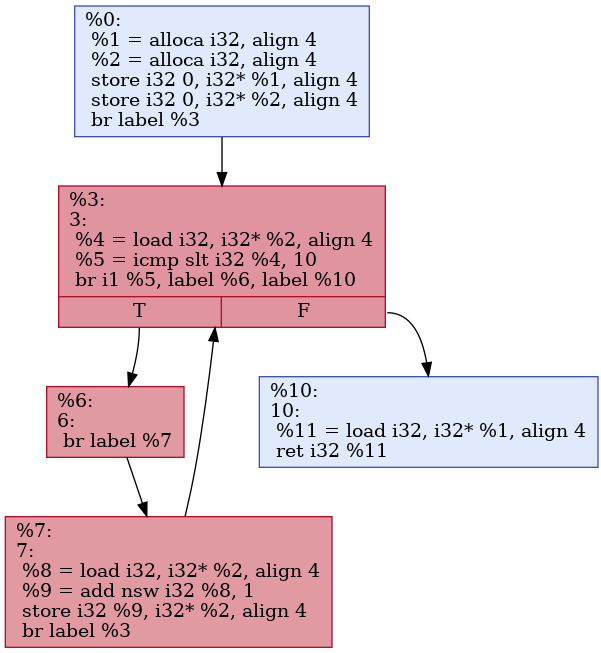
\includegraphics[scale=.70]{Figures/05/simple-loop.png}}
    \caption{Simple Loop Basic Block.} 
    \label{fig:simple-loop-bb}
\end{figure}

The first step to get the offline measurement is to inline the code in the basic
block. In this simple program, we cannot inline the code further, because there
is no function call at all. 

After we inline the code, we traverse the basic block and use heuristic to
marks some basic blocks to some checkpoints types. The next step, the
measurement extractor traverse each path between two checkpoints and collect the
list of action between them. We show the visual of measurement result in
Figure~\ref{fig:simple-loop-loa}.

\begin{figure}[ht]
    \centerline{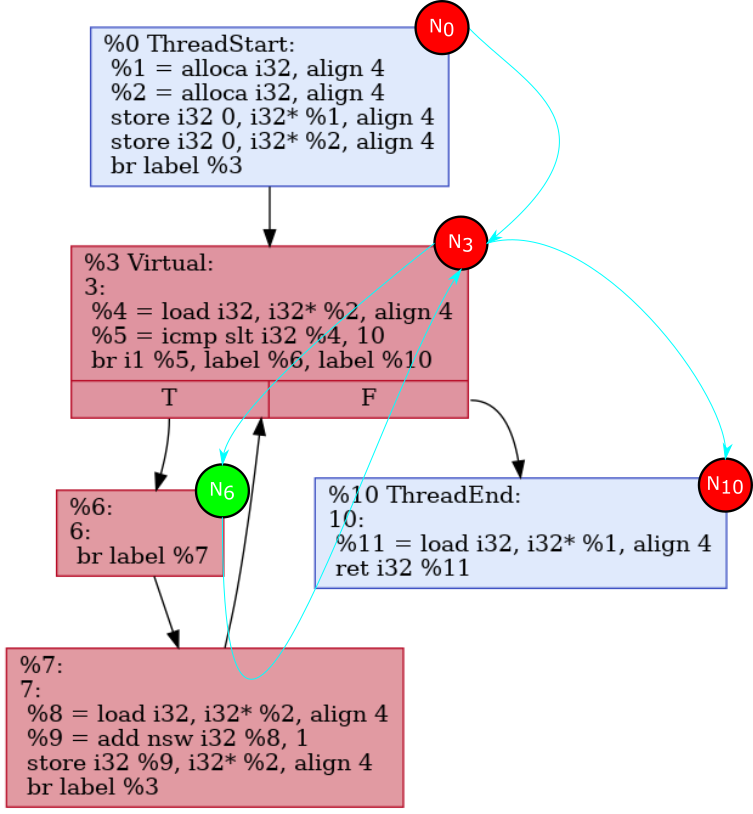
\includegraphics[scale=.60]{Figures/05/simple-loop-loa.png}}
    \caption{Simple Loop Checkpoints and LoAs.} 
    \label{fig:simple-loop-loa}
    \vspace{20cm}
\end{figure}

The actual measurement between the checkpoints is the following. In summary,
this program has 5 lines of source code and around 39 IR source lines. The
program has 5 basic blocks, 4 LoAs and 4 measurements.

\begin{align*}  
    N_0 - N_3 &\Rightarrow [] \\
    N_3 - N_3 &\Rightarrow [N_3, N_6] \\
    N_3 - N_{10} &\Rightarrow [N_3, N_{10}] \\
\end{align*}
